\documentclass{jarticle}
\usepackage{robomech}
\usepackage{graphicx}

\begin{document}
\makeatletter
\title{未知障害物環境に対応するための\\モンテカルロ自己位置推定における観測範囲の選択}
{―まだ決まってない―}
{Observation Range Selection in Monte Carlo localization for Unknown Obstacle Environments}
{-Not decided yet.-}

\author{
\begin{tabular}{ll}
 ○学\hspace{1zw} 池邉龍宏(千葉工大)& 正\hspace{1zw}林原靖男\hspace{1zw} (千葉工大)\\
 \hspace{1zw}正\hspace{1zw}上田隆一(千葉工大)\\
 % ※協賛・後援団体の会員資格で発表される場合は「正・学」は不要です。
 \end{tabular}
 % &\\
 \vspace{1zh} \\
 \begin{tabular}{l}
{\small Tatsuhiro IKEBE, Chiba Institute of Technology, 
 }\\
 {\small Yasuo HAYASHIBARA, Chiba Institute of Technology}\\
 {\small Ryuichi UEDA, Chiba Institute of Technology}\\
\end{tabular}
}
\makeatother

\abstract{ \small 
Not decided yet.
}

\date{} % 日付を出力しない
\keywords{Autonomous mobile robots, Navigation, LiDAR Localization, MCL, Unknown Obstacle}

\maketitle
\thispagestyle{empty}
\pagestyle{empty}

\small
\section{緒言(大見出し:ゴシック体・10pt・\protect\\ 強調文字・中央寄せ)}%===========================
本文:明朝体・9pt(欧文Times New Roman, 9pt)、文字間隔は1行26文字程度、行間隔は4.2mm程度にして下さい。

\subsection{論文作成に関する注意事項を以下に示します。(中見出し:ゴシック体・9pt・強調文字・左寄せ)}%-----------
\begin{itemize}
	\item 用紙サイズ:A4(210×297mm)とします。
	\item 用紙マージン:上下25mm。日本語表題から\textbf{\textit{Key Words}}までの1段組の部分は、左右25mm以上空けて下さい。本文からは2段組とし、左右15mm、段間は6mmとします。
	\item 文字のフォント、大きさ:\reftab{tbl: table1}を参照下さい。
	\item 図の画質:300dpi以上の画質の高いものにして下さい。
	\item 図・表のタイトル:図のタイトルには「Fig.\# English title」、表のタイトルには「Table \# English title」という形式を用い、文中ではそれぞれ「図\#」、「表\#」という表現にして下さい。
	\item グラフの軸タイトル:各軸のタイトルに変数記号だけを記述するのは避けて下さい。\reffig{fig: fig1}に示すように、軸を表す語句ならびに単位を記入して下さい。
	\item 式:以下に示すように、右寄せで番号をふり、式は中央に配置して下さい。文中では「\refeqn{eqn: eq1}」と表現して下さい。
	
	\begin{equation}
		M\ddot{r}_{str1} + F_{frk} = Mg
		\label{eqn: eq1}
	\end{equation}

	\item 単位:SI単位系とします。
	\item 本文中に文献を引用する場合、引用を表す語句や文の後ろに文献番号(例えば\cite{Shinjuku98})を振って下さい。文献を主語や目的語などに用いる場合、「文献\cite{Shinjuku98}では、・・」などのようにして、番号のみの表現を避けて下さい。
	\item 連名の場合には講演発表者氏名の前に○印をつけて下さい。
	\item 作成した論文はPDFファイル形式に変換し、PDFファイルのみを学会本部へ提出して下さい。PDFファイルの提出は本講演会ホームページ記載のアップロードのページの指示に従って下さい。
	\item[]
	\item[※] ただし、PDFファイルの容量は2MB以下、論文のページ数は2頁以上4頁以下とします。なお、印刷原稿の提出は不要ですので、郵送しないで下さい。
	\item[※] 講演番号、講演会名、ページ番号は記載しないようにして下さい。
\end{itemize}

%※ ただし、PDFファイルの容量は2MB以下、論文のページ数は2頁以上4頁以下とします。なお、印刷原稿の提出は不要ですので、郵送しないで下さい。

%※ 講演番号、講演会名、ページ番号は記載しないようにして下さい。


\begin{table}[h]
 \caption{Type size and typefaces for papers}
 \label{tbl: table1}
 \centering
 \footnotesize
 \begin{tabular}{|p{7zw}|c|c|c|}
  \hline
	適用場所	&日本語	&欧文 \\\hline
	標準のフォント	&明朝体 9pt	&Times New Roman 9pt \\\hline
	日本語表題	&ゴシック体 14pt	&Arial 14pt \\\hline
	日本語副表題	&ゴシック体 12pt	&Arial 12pt \\\hline
	英語表題	&-&Times New Roman 12pt \\\hline
	英語副表題	&-&Times New Roman 10pt \\\hline
	日本語著者名	&明朝体 10pt &-\\\hline
	英語著者名	&-&Times New Roman 9pt \\\hline
	アブストラクト・キーワード	&-&Times New Roman 9pt \\\hline
	大見出し	&ゴシック体 10pt	&Arial 10pt \\\hline
	中見出し	&ゴシック体 9pt	&Arial 9pt \\\hline
	図・表の番号・タイトル	 &-&Times New Roman 9pt \\\hline
	文献	&明朝体 8pt	&Times New Roman 8pt \\
  \hline
 \end{tabular}
\end{table}

\begin{figure}[h]
 \centering
  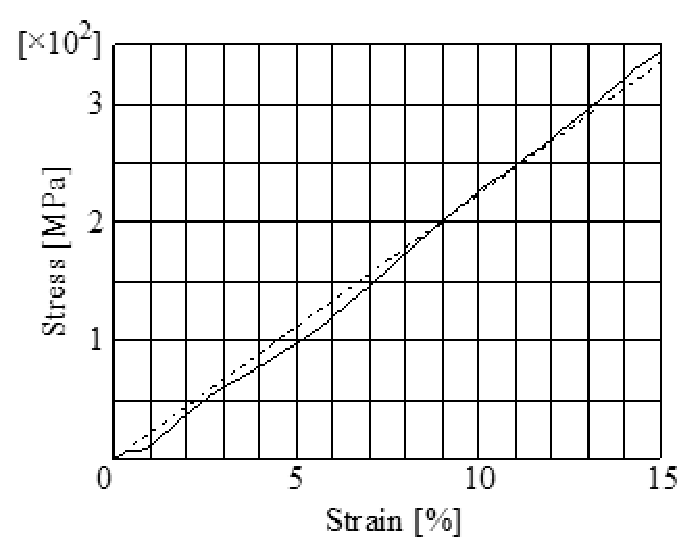
\includegraphics[height=38mm]{fig1.eps}
  \vspace*{-4mm}
  \caption{Tensile stress-strain diagram}
  \label{fig: fig1}
\end{figure}


\footnotesize
\begin{thebibliography}{99}

\bibitem{Shinjuku98}
新宿大五朗,渋谷次郎,東京 学,``キャスティングマニピュレーションに関する研究(第1報,可変長の紐状柔軟リンクを有するマニピュレータの提案とそのスイング制御法)'',{\it 機論C編}, vol.64-626, pp.3854--3861, 1998.

\bibitem{Shinjuku99}
Shinjuku, D., Shibuya, J. and Tokyo, M., ``Swing Motion Control of Casting Manipulation,'' {\it IEEE Control Systems}, vol.19-4, pp.56--64, 1999.

\end{thebibliography}

\normalsize
\end{document}
